\documentclass[%
  pdftex,%            Weiterreichen des gewählten Backend-Treibers für pdfTeX %
  a4paper,
  11pt,%                                          Größe der Grundschrift 11pt %
  oneside,%                                                zweiseitiger Druck %
  BCOR = 1cm,%                                                 Bindekorrektur %
  cleardoublepage=plain,%               Kapitelanfang immer auf rechter Seite %
  fleqn,%                                       Gleichungen links, eingerückt %
  numbers=noenddot,%                         Kapitel-Nummerierung ohne Punkte %
  headings=normal,%                                 normalgroße Überschriften %
  bibliography=totocnumbered,%                  Literaturverszeichnis ins TOC %
  listof=numbered,%               Abbildungs- und Tabellenverzeichnis ins Toc %
  ngerman,%             Weiterreichen "Neue Rechtschreibung" an weiter Pakete %
  headsepline=0.08em,%
]{scrbook}%                   DiplA aufgebaut auf der Koma-Script Buch-Klasse %

%%%%%%%%%%%%%%%%%%%%%%%%%%%%%%%%%%%%%%%%%%%%%%%%%%%%%%%%%%%%%%%%%%%%%%%%%%%%%%%
%                                                                             %
%          layout.tex - Pakete, Layout- und Formatierungsanweisungen          %
%                                                                             %
%%%%%%%%%%%%%%%%%%%%%%%%%%%%%%%%%%%%%%%%%%%%%%%%%%%%%%%%%%%%%%%%%%%%%%%%%%%%%%%

\usepackage[utf8]{inputenc}%                       verwendetes Input Encoding %
\usepackage[TS1,T1]{fontenc}%                       verwendete Font Encodings %
\usepackage{csquotes}%                                      Anführungszeichen %
\usepackage{amsmath,amsfonts,amssymb}%   AMS Mathematik-Hilfsmittel für LaTeX %
\usepackage{esvect}%                                      Schöne Vektorpfeile %
\usepackage{textcomp}%                 Unterstützung der Text Companion Fonts %
\usepackage[pdftex]{graphicx}%           Unterstützung für Graphik-Einbindung %
\usepackage[pdftex,hyperref,cmyk,dvipsnames]{xcolor}%          Treiber-unabhängige Farb- % 
%                                        erweiterungen für LaTeX und pdfLaTeX %
% \definecolor{uniblue}{cmyk}{1 0.72 0 0.38}%       Farbdefinition des Uni-Blau %
% \definecolor{diplaBlue}{cmyk}{1 0.8 0 0}%                "       schönes Blau %

\usepackage{array}%     erweiterte Implementierung der array und tabular Umg. %
\usepackage{tabularx}%     Ausdehnung von Tabellen auf eine definierte Breite %
\usepackage{colortbl}%                     erlaubt farbige Zeilen und Spalten %
\usepackage{booktabs}%               typographisch "schöne" Tabellen in LaTeX %
\usepackage{longtable}%                                        lange Tabellen %
\usepackage{setspace}%       Festlegung von unterschiedlichen Zeilenabständen %
\usepackage{scrlayer-scrpage}%             Neuere Version der scrpage2 Klasse %
\usepackage{xspace}%                definiert Befehle "that don't eat spaces" %
\usepackage[german]{datenumber}%       Konvertierung zwischen Datum <--> Zahl %
\usepackage[ngerman]{babel}

\usepackage{xfrac} %               Typographisch korrekte Brüche im Fließtext %
\usepackage{changes}

\usepackage{ulem}% Durchstreichung %

\usepackage[%
   pdftex,%                                                     Backend Driver %
   colorlinks          = true,%                   Färbung von Links und Ankern %
  linkcolor           = black!70,%               Farbe für normale interne Links %
%   anchorcolor         = black,%                          Farbe für Anker-Text %
%   citecolor           = black,%           Farbe für Literaturhinweise im Text %
%   filecolor           = black,%             Farbe für URLs zu lokalen Dateien %
%   menucolor           = black,%               Farbe für Acrobat Menü-Einträge %
%   pagecolor           = gray,%             Farbe für Links zu anderen Seiten %
   urlcolor            = blue,%                        Farbe für verinkte URLs %
   pdfstartview        = {FitH},%         Festlegung der Startup-Seitenansicht %
   pdfpagelabels,%                                                             %
   pdfpagelayout       = {SinglePage},%           Festlegung der Layoutansicht %
   bookmarksopen       = true,%         Anzeige von Bookmarks, falls verwendet %
   bookmarksopenlevel  = 1,%      Tiefe, bis zu der Bookmarks angezeigt werden %
   bookmarksnumbered   = true,%                                                %
   breaklinks,%                               Links »überstehen« Zeilenumbruch %
   plainpages          = false,%     notwendig wg. der Seiten(neu)nummerierung %
%                        von Vorspann und Haupttext, andernfalls pdf-Warnungen %
]{hyperref}

\usepackage{hypcap}%                              Legt den Anker für pdf-link %
%                     auf den Anfang eines Bildes, nicht auf die Unterschrift %

\usepackage[
    printonlyused
]{acronym}
\usepackage[section]{placeins}


\usepackage[titles]{tocloft}%              individuelle Formatierungen am TOC %

%-----------------------------------------------------------------------------%
%              andere Schriftauswahl statt der Standardschriften, siehe dazu: %
%                                       http://home.vr-web.de/~was/fonts.html %
%------------------------------------------------------------------------------
\usepackage{mathptmx}%                 Times als Grund- und Mathematikschrift %
%\usepackage{mathpazo}%              Palatino als Grund- und Mathematikschrift %
\usepackage[scaled=0.9]{helvet}%   Helvetica (psnfss) als serifenlose Schrift %
\renewcommand{\bfdefault}{b}%
\usepackage[scaled=0.9]{beramono}%              freie Bitstream-Familie Bera, %
%                                daraus die Monospaced als Typewriter-Schrift %
%-----------------------------------------------------------------------------%
%     diverse Pakete, z.B. microtype für pdfTeXs micro-typographic extensions %
%-----------------------------------------------------------------------------%
\usepackage[stretch=15,shrink=15,step=5]{microtype}
\usepackage{dirtree, ellipsis, fixltx2e, mparhack}
%-----------------------------------------------------------------------------%
%                                Einheitliche Formatierung für Unterschriften %
%-----------------------------------------------------------------------------%
\usepackage[
	format        = hang,
	justification = RaggedRight,
	position      = below,
	width         = .9\textwidth
]{caption}
\usepackage{subcaption}%       Neueres Paket zur Unterstützung von Subfigures %

%-----------------------------------------------------------------------------%
%                                                    Quelltext-Formatierungen %
%-----------------------------------------------------------------------------%
\usepackage{listings}
\lstset{
    language=c++,         % Sourcecode language ist C++
    numbers=none,            % No linenumbers
%    stepnumber=1,            % Every line got his own number.
    numbersep=5pt,           % 5pt distance to Sourcecode
    numberstyle=\tiny,       % tiny numbers.
    breaklines=true,         % break lines if it has to do.
    breakautoindent=true,    % Nach dem Zeilenumbruch Zeile einrücken.
    postbreak=\space,        % Bei Leerzeichen umbrechen.
    tabsize=2,               % Tabulatorsize 2
    basicstyle=\ttfamily\footnotesize, % Nichtproportionale Schrift, klein für den Quellcode
    showspaces=false,        % Leerzeichen nicht anzeigen.
    showstringspaces=false,  % Leerzeichen auch in Strings ('') nicht anzeigen.
    extendedchars=true,      % Alle Zeichen vom Latin1 Zeichensatz anzeigen.
    backgroundcolor=\color{black!5}, % Hintergrundfarbe des Quellcodes setzen.
    captionpos=b,         % Caption unter und nicht über das Listing schreiben
    frame = lines,
	floatplacement = tb,
	morekeywords = {foreach},
    %rulesepcolor=\color{darkgrey}
} 
%-----------------------------------------------------------------------------%
%                                                        Schrifteinstellungen %
%------------------------------------------------------------------------------
%\linespread{1.25}\selectfont%                                    mehr Abstand %
\linespread{1.10}\selectfont%                                    mehr Abstand %

%   Redefinition Typewriter-Befehls: kleinere Schrift, Silbentrennungszeichen %
\renewcommand\texttt[1]{% 
\small\ttfamily\hyphenchar\font=\defaulthyphenchar#1{}\normalsize\rmfamily\hyphenchar\font=\defaulthyphenchar}

\setkomafont{sectioning}{%        Abschnittsüberschriften serifenlos und fett %
\sffamily\bfseries}

\addtokomafont{caption}{%                            Bildunterschriften klein %
\normalfont\normalcolor\small}

\addtokomafont{captionlabel}{\small\bfseries}%             Bezeichnungen fett %


%------------------------------------------------------------------------------
%                             individuelle Formatierungen an TOC, LOF und LOT %
%------------------------------------------------------------------------------
\renewcommand{\cftchapfont}{%
\sffamily\bfseries}%                       Kapitelbezeichnung fett & serifenlos
\renewcommand{\cftchappagefont}{\sffamily
\bfseries}%                                     Kapitelnummer fett & serifenlos
\setlength{\cftbeforesecskip}{1.5pt}%           vert. Abstand vor Abschnittsbez.
\setlength{\cftbeforesubsecskip}{1pt}%     vert. Abstand vor Unterabschnittsbez.
\cftsetindents{chapter}{0em}{1.3em}%                         Einzug für Kapitel
\cftsetindents{section}{1.3em}{2em}%                      Einzug für Abschnitte
\cftsetindents{subsection}{3.3em}{2.7em}%            Einzug für Unterabschnitte
\cftsetindents{subsubsection}{6em}{3.3em}%           Einzug für Unterabschnitte


\setlength{\cftbeforetabskip}{1.5pt}%   vert. Abstand vor Tabellenbezeichnungen
\cftsetindents{table}{0em}{2.5em}%            Einzüge für Tabellenbezeichnungen
\renewcommand{\cfttabpresnum}{\hfill}%
\renewcommand{\cfttabaftersnum}{\hspace*{0.6em}}%

\setlength{\cftbeforefigskip}{1.5pt}%             Abstand vor Bildbezeichnungen
% \setlength{\cftbeforesubfigskip}{0.5pt}%     Abstand vor Unterbildbezeichnungen
% \cftsetindents{figure}{0em}{2.5em}%               Einzüge für Bildbezeichnungen
% \cftsetindents{subfigure}{2.5em}{1.8em}%     Einzüge für Unterbildbezeichnungen
% \renewcommand{\cftfigpresnum}{\hfill}%
\renewcommand{\cftfigaftersnum}{\hspace*{0.6em}}%

%-----------------------------------------------------------------------------%
%                                 Einstellung bestimmter Längen und Parameter %
%-----------------------------------------------------------------------------%
%\parindent0mm%                     KEIN Einzug bei neuem Absatz, statt dessen %
%\parskip2mm plus1.5pt minus1.5pt%              Abstand zwischen zwei Absätzen %
%\parindent5mm%                                        Einzug bei neuem Absatz %

%                 zusätzlicher vertikaler Abstand vor und nach Gleitobjekten, %
%                                    die mit der Option "h" eingefügt werden: %
\setlength{\intextsep}{1.5\baselineskip plus 2pt minus 2pt}%

%                           zusätzlicher vertikaler Abstand für Gleitobjekte, %
%                         die mit den Optionen "t" bzw. "b" eingefügt werden: %
\setlength{\textfloatsep}{1.5\baselineskip plus 2pt minus 2pt}

%\setcapwidth[c]{.8\textwidth}%    Abbildungsbeschriftungen 80% der Textbreite %

\addtolength{\footnotesep}{2pt}%      mehr Abstand zwischen Fußnoten und Text %

\pagestyle{scrheadings}%               Seitenstil mit lebenden Kolumnentiteln %
\clearpairofpagestyles
\ohead[]{\headmark}
\cfoot[]{}
\ofoot[\pagemark]{\pagemark}
% \setheadsepline{0.08em}%    Einstellungen der Dicke der Kopfzeilen-Trennlinie %

\setcounter{secnumdepth}{3}%                               Nummerierungstiefe %
\setcounter{tocdepth}{2}%                  Inhaltsverzeichnis bis zur Tiefe 2 %
\setcounter{lofdepth}{2}%               Abbildungsverzeichnis bis zur Tiefe 2 %

\renewcommand{\topfraction}{0.9}%      Anteile der Seite, die maximal/minimal %
\renewcommand{\bottomfraction}{0.9}%    von Abbildungen bzw. Text eingenommen %
\renewcommand{\textfraction}{0.1}%                              werden können %


%------------------------------------------------------------------------------
%                  Einstellungen für den Zeilenumbruchsalgorithmus, siehe dazu:
%           --> http://www.jr-x.de/publikationen/latex/tipps/zeilenumbruch.html
%------------------------------------------------------------------------------
\emergencystretch 1.5em%
\clubpenalty = 10000%
\widowpenalty = 10000%
\displaywidowpenalty = 10000
\doublehyphendemerits = 10000%
\tolerance=500

\hfuzz 0.25pt%                     Grenze, ab der "overfull hbox" gemeldet wird
\vfuzz \hfuzz%                     Grenze, ab der "overfull vbox" gemeldet wird

%------------------------------------------------------------------------------
%                              Einstellungen des Satzspiegels mit den Vorgaben:
%                  Rand innen: 35mm, Rand außen 25 mm, Rand oben/(unten) ~25 mm
%------------------------------------------------------------------------------

%%\paperwidth    597.50787pt%                            597,50787 pt = 210,00 mm
%%\paperheight   845.04684pt%                            845,04684 pt = 297,00 mm
%%\paperwidth    210mm
%%\paperheight   297mm
%%\textwidth     426.79135pt%       210 - 35 - 25 mm  =  426,79135 pt = 150,00 mm
%\textwidth 140mm
%%\textheight    638.40076pt%        41 Zeilen           621,07825 pt = 218,28 mm
%%\oddsidemargin  27.31465pt%                             27,31465 pt =   9,60 mm
%%\evensidemargin -1.13811pt%                              1,13811 pt =  -0,40 mm
%%\oddsidemargin  10mm
%%\evensidemargin 8.5mm
%\topmargin      -8.53583pt%                              8,53583 pt =  -3,00 mm
%\headheight     17.07165pt%                             17,07165 pt =   6,00 mm
%\headsep        19.91692pt%                             19,91692 pt =   7,00 mm
%\footskip       45.52440pt%                             45,52440 pt =  16,00 mm
%\marginparwidth 59.75079pt%                             59,75079 pt =  21,00 mm
%\marginparsep    8.53583pt%                              8,53583 pt =   3,00 mm
%\skip\footins  10.8pt plus 4.0pt minus 2.0pt
%%\hoffset 0.0pt%
%%\voffset 0.0pt%

\usepackage{todonotes}

% FOM-"Standard"
% \usepackage[style=verbose-trad2, backend=biber]{biblatex}
% \counterwithout*{footnote}{chapter}
% \AtEveryCitekey{%
% \clearfield{url}%
% \clearfield{isbn}%
% \clearfield{doi}%
% }
% Stern (IEEE)
\usepackage[style=ieee, mincitenames=1, maxcitenames=2, backend=biber]{biblatex}
\usepackage{xurl}%      URLs werden so auch im Literaturverzeichnis umgebrochen %

% \citetitle: Titel mit deutschen Anführungszeichen
\DeclareFieldFormat*{citetitle}{\glqq#1\grqq}

% "et al." für die Abkürzung mehrerer Autoren verwenden
\DefineBibliographyStrings{german}{%
  andothers = {\emph{et al}\adddot}
}

% Hier die entsprechende .bib-Datei eintragen
\addbibresource{seminar-lit.bib}

% Keine Warnung für geteilte Bibliographien
\BiblatexSplitbibDefernumbersWarningOff
\defbibheading{bibintoc}[\bibname]{%
  \addchap{#1}}
%%%%%%%%%%%%%%%%%%%%%%%%%%%%%%%%%%%%%%%%%%%%%%%%%%%%%%%%%%%%%%%%%%%%%%%%%%%%%%%
%                                                                             %
%               commands.tex - eigene Befehle für diverse Dinge               %
%                                                                             %
%%%%%%%%%%%%%%%%%%%%%%%%%%%%%%%%%%%%%%%%%%%%%%%%%%%%%%%%%%%%%%%%%%%%%%%%%%%%%%%

%-----------------------------------------------------------------------------%
%                                                   Grundlegende Definitionen %
%-----------------------------------------------------------------------------%
\author{Fabian Donatus Wolfgang Urbanek}
\newcommand{\daAutor}{Fabian Donatus Wolfgang Urbanek}
\newcommand{\daMatrikelnummer}{667074}
\newcommand{\daTitel}{Konzeption, Implementierung und Evaluation eines Virtual-Tabletop-Plugins für Obsidian.md}
\newcommand{\daTitelEins}{Konzeption, Implementierung und Evaluation}
\newcommand{\daTitelZwei}{eines Virtual-Tabletop-Plugins für Obsidian.md}
\newcommand{\daTitelDrei}{}
\newcommand{\daUnternehmen}{Unternehmen GmbH \& Co. KG}

\newcommand{\daUniURL}{http://www.fom.de}
\newcommand{\daUniLogo}[1]{
\includegraphics[#1]{./bilder/FOM}}
\newcommand{\daStudiengang}{Bachelor Wirtschaftsinformatik}

\newcommand{\daAutorAdresse}{Hinter der Höh 20}
\newcommand{\daAutorPLZ}{34630}
\newcommand{\daAutorOrt}{Gilserberg}

\newcommand{\daDate}{01.01.2026}


\newcommand{\daGutachterEins}{Prof. Dr. Claudius Stern}

%-----------------------------------------------------------------------------%
%                                                   einige Mathe-Definitionen %
%-----------------------------------------------------------------------------%
\newcommand{\CoG}{\operatorname{CoG}}

%-----------------------------------------------------------------------------%
%                                                  Befehl für das BibTeX-Logo %
%-----------------------------------------------------------------------------%
\makeatletter
\DeclareRobustCommand{\BibTeX}{B\hbox{\check@mathfonts
\fontsize\sf@size\z@
\math@fontsfalse\selectfont
IB}\kern-.08em
\TeX}
\makeatother

%-----------------------------------------------------------------------------%
%      Punktereihe mit größerem Abstand zwischen den Punkten als bei \dotfill %
%-----------------------------------------------------------------------------%
\makeatletter
\def\punktfill{\cleaders\hbox{$\m@th \mkern4mu . \mkern4mu$}\hfill}
\makeatother

%-----------------------------------------------------------------------------%
%                                    Makros zur Festlegung von PDF-Attributen %
%-----------------------------------------------------------------------------%
\newcommand{\setPDFCreationDate}{%               CreationDate ist Abgabedatum %
\pdfinfo{%
/CreationDate (D:%
\thedateyear%
\ifnum\value{datemonth}<10 0\fi%
\thedatemonth%
\ifnum\value{dateday}<10 0\fi%
\thedateday%
010000+01'00')}%
}
%-----------------------------------------------------------------------------%
\newcommand{\setPDFModDateToCreationDate}{% ModDate ist ebenfalls Abgabedatum %
\pdfinfo{/CreationDate (D:\thedateyear%
\ifnum\value{datemonth}<10 0\fi\thedatemonth%
\ifnum\value{dateday}<10 0\fi\thedateday010000+01'00')}}
%-----------------------------------------------------------------------------%


\gdef\twodigits#1{\ifnum#1<10 0\fi\the#1}
%-----------------------------------------------------------------------------%
\newcommand{\setPDFModDateToCurrentDate}{%        ModDate ist aktuelles Datum
\begingroup
\count0=\time \divide\count0 by 60
\edef\x{\twodigits{\count0}}%
\multiply\count0 by 60
\count1=\time \advance\count1 by -\count0
\edef\x{\x\twodigits{\count1}}%
\edef\x{/ModDate (D:\the\year 
\twodigits\month \twodigits\day \x 00+01'00')}%
\expandafter\endgroup
\expandafter\pdfinfo\expandafter{\x}%
}

%-----------------------------------------------------------------------------%
%                  Titel, Thema, Author, Schlüsselwörter und Erzeugerprogramm %
%-----------------------------------------------------------------------------%
\newcommand{\daHyperSetup}{%
\hypersetup{%
pdftitle    = {\protect{\daTitel}},%
pdfsubject  = {Diplomarbeit an der Universität Paderborn},%
pdfauthor   = {\protect{\daAutor}},%
pdfkeywords = {\daPDFKeywords},%
pdfcreator = {LaTeX2e mit {\frqq KOMA-Script\flqq} Book-Klasse und {\frqq hyperref\flqq}-Package}}
}
%-----------------------------------------------------------------------------%
%          Befehle für bestimmte deutsche Abkürzungen mit passenden Abständen %
%                                         (kein Anspruch auf Vollständigkeit) %
%-----------------------------------------------------------------------------%
\newlength{\abkz}
\setlength{\abkz}{1pt}
\newcommand{\abkrz}{\hspace{\abkz}}

\newcommand{\bzw}{bzw.\@\xspace}
\newcommand{\bzgl}{bezüglich\@\xspace}
\newcommand{\ca}{ca.\@\xspace}
\newcommand{\dah}{\mbox{d.{\abkrz}h.}\@\xspace}
\newcommand{\Dah}{D.{\abkrz}h.\@\xspace}
\newcommand{\ds}{d.{\abkrz}s.\@\xspace}
\newcommand{\evtl}{evtl.\@\xspace}
\newcommand{\etc}{etc.\@\xspace}
\newcommand{\ua}{u.{\abkrz}a.\@\xspace}
\newcommand{\Ua}{U.{\abkrz}a.\@\xspace}
\newcommand{\usw}{usw.\@\xspace}
\newcommand{\va}{v.{\abkrz}a.\@\xspace}
\newcommand{\vgl}{vgl.\@\xspace}
\newcommand{\zB}{\mbox{z.{\abkrz}B.}\@\xspace}
\newcommand{\ZB}{Zum Beispiel\xspace}
\newcommand{\zT}{z.{\abkrz}T.\@\xspace}
\newcommand{\ZT}{Zum Teil\xspace}
\newcommand{\zZ}{zur Zeit\xspace}
\newcommand{\sa}{s.{\abkrz}a.\@\xspace}
\newcommand{\ia}{i.{\abkrz}a.\@\xspace}
\newcommand{\uU}{u.{\abkrz}U.\@\xspace}
\newcommand{\bspw}{beispielsweise\@\xspace}
\newcommand{\Bspw}{Beispielsweise\@\xspace}
\newcommand{\ggf}{gegebenenfalls\@\xspace}
\newcommand{\sog}{sogenannte\@\xspace}
\newcommand{\soger}{sogenannter\@\xspace}
\newcommand{\sogen}{sogenannten\@\xspace}
\newcommand{\soges}{sogenanntes\@\xspace}
\newcommand{\og}{o.\,g.\@\xspace}

%-----------------------------------------------------------------------------%
%        erzeugt eingeklammerten, kursiven Begriff mit dem Wort "engl." davor %
%-----------------------------------------------------------------------------%
\newcommand{\engl}[1]{%
(engl. \emph{#1})\@\xspace}%

%-----------------------------------------------------------------------------%
%                    Befehle für das Verzeichnis der Akronyme und Abkürzungen %
%-----------------------------------------------------------------------------%
\newlength{\acronWidth}
\newcommand{\acron}[2]{%
\protect\hyperdef{acDef}{#1}{\rule{0pt}{1pt}}\\[-3ex]%
\makebox[\acronWidth][l]{#1}~~{#2}\par%
}
\newcommand{\acronShort}[1]{\protect\hyperlink{acDef.#1}{#1}}
\newcommand{\acronShortPlural}[1]{\protect\hyperlink{acDef.#1}{#1{s}}}


%-----------------------------------------------------------------------------%
%                         Neudefinition der Referenzierungs-Befehle (kleiner) %
%-----------------------------------------------------------------------------%
%\makeatletter\renewcommand{\@cite}[2]{[{\small #1\if@tempswa , #2\fi}]}\makeatother
%\makeatletter\renewcommand{\@biblabel}[1]{[{\small #1}]}\makeatother

%-----------------------------------------------------------------------------%
%   Gestaltung des Datei-Verweises zur CD-ROM, falls BibTeX-Item cdlink = {1} %
%                                         (siehe dazu die BibTeX-Style-Datei) %
%-----------------------------------------------------------------------------%
\newcommand{\CDLink}[1]{%
~\mbox{$\rightarrow$ {\itshape\footnotesize %
Auf beiliegender CD:}~~\href{file:./literatur/#1}{%
\raisebox{-0.5pt}{\includegraphics[height=7.5pt]{cdIconBlue}}%
\textcolor{diplaBlue}{\ttfamily\footnotesize/literatur/#1.pdf}}}}

%-----------------------------------------------------------------------------%
\newcommand{\blindtext}{%                                eigener Blindtext ;) %
%-----------------------------------------------------------------------------%
Weit hinten, hinter den Wortbergen, fern der Länder Vokalien und 
Konsonantien leben die Blindtexte. Abgeschieden wohnen sie in 
Buchstabhausen an der Küste des Semantik, eines großen Sprachozeans. 
Ein kleines Bächlein namens Duden fließt durch ihren Ort und versorgt 
sie mit den nötigen Regelialien. Es ist ein paradiesmatisches Land, 
in dem einem gebratene Satzteile in den Mund fliegen. Nicht einmal 
von der allmächtigen Interpunktion werden die Blindtexte 
beherrscht -- ein geradezu unorthographisches Leben. 

Eines Tages aber beschloß eine kleine Zeile Blindtext, 
ihr Name war Lorem Ipsum, hinaus zu gehen in die weite Grammatik. 
Der große Oxmox riet ihr davon ab, da es dort wimmele von bösen Kommata, 
wilden Fragezeichen und hinterhältigen Semikola, doch das Blindtextchen 
ließ sich nicht beirren. Es packte seine sieben Versalien, schob sich 
sein Initial in den Gürtel und machte sich auf den Weg. 
Als es die ersten Hügel des Kursivgebirges erklommen hatte, warf es 
einen letzten Blick zurück auf die Skyline seiner Heimatstadt Buchstabhausen, 
die Headline von Alphabetdorf und die Subline seiner eigenen Straße, 
der Zeilengasse. Wehmütig lief ihm eine rhetorische Frage über die Wange, 
dann setzte es seinen Weg fort. Unterwegs traf es eine Copy. Die Copy 
warnte das Blindtextchen, da, wo sie her käme wäre sie zigmal umgeschrieben 
worden und alles, was von ihrem Ursprung noch übrig wäre, sei das Wort "`und"' 
und das Blindtextchen solle umkehren und wieder in sein eigenes, sicheres Land 
zurückkehren. Doch alles Gut zureden konnte es nicht überzeugen und so dauerte 
es nicht lange, bis ihm ein paar heimtückische Werbetexter auflauerten, es mit 
Langue und Parole betrunken machten und es dann in ihre Agentur schleppten, 
wo sie es für ihre Projekte wieder und wieder mißbrauchten. Und wenn es nicht 
umgeschrieben wurde, dann benutzen sie es immer noch.%
}



%=============================================================================%
%                                 Befehle zum Setzen eines Verzeichnis-Baumes %
%=============================================================================%
\newcounter{dirCounter}
\newcommand{\cdIcon}[1]{%
\raisebox{-2pt}{\includegraphics[width=10pt]{cdIcon}}~%
{\ttfamily\bfseries\itshape\small #1}\@\xspace
}
%-----------------------------------------------------------------------------%
%                                     Befehle für Ordner/Dateien auf 1. Ebene %
%-----------------------------------------------------------------------------%
%                                offener Order mit mit Folgemuster:  E        %
%-----------------------------------------------------------------------------%
\newcommand{\oEm}[2][21]{%
\begin{picture}(12,6)
  \linethickness{.6pt}
  \put(5,-6){\line(0,1){#1}}
  \put(5,3){\line(1,0){5}}
  \put(5,3){\makebox(0,0){\includegraphics[width=5pt]{minus}}}
\end{picture}%
\raisebox{-0.5pt}{\includegraphics[width=12pt]{oOrdner}}~%
{\ttfamily\bfseries\itshape\footnotesize #2}\@\xspace
}
%-----------------------------------------------------------------------------%
%                          geschlossener Order mit mit Folgemuster:  E        %
%-----------------------------------------------------------------------------%
\newcommand{\oEp}[2][21]{%
\begin{picture}(12,6)
  \linethickness{.6pt}
  \put(5,-5){\line(0,1){#1}}
  \put(5,3){\line(1,0){5}}
  \put(5,3){\makebox(0,0){\includegraphics[width=5pt]{plus}}}
\end{picture}%
\raisebox{-0.5pt}{\includegraphics[width=12pt]{ordner}}~%
{\ttfamily\bfseries\itshape\footnotesize #2}\@\xspace
}
%-----------------------------------------------------------------------------%
%                                    offener Order mit Folgemuster:  L        %
%-----------------------------------------------------------------------------%
\newcommand{\oLm}[2][13]{%
\begin{picture}(12,6)
  \linethickness{.6pt}
  \put(5,3){\line(0,1){#1}}
  \put(5,3){\line(1,0){5}}
  \put(5,3){\makebox(0,0){\includegraphics[width=5pt]{minus}}}
\end{picture}%
\raisebox{-0.5pt}{\includegraphics[width=12pt]{oOrdner}}~%
{\ttfamily\bfseries\itshape\footnotesize #2}\@\xspace
}
%-----------------------------------------------------------------------------%
%                              geschlossener Order mit Folgemuster:  L        %
%-----------------------------------------------------------------------------%
\newcommand{\oLp}[2][13]{%
\begin{picture}(12,6)
  \linethickness{.6pt}
  \put(5,3){\line(0,1){#1}}
  \put(5,3){\line(1,0){5}}
  \put(5,3){\makebox(0,0){\includegraphics[width=5pt]{plus}}}
\end{picture}%
\raisebox{-0.5pt}{\includegraphics[width=12pt]{ordner}}~%
{\ttfamily\bfseries\itshape\footnotesize #2}\@\xspace
}
%-----------------------------------------------------------------------------%
%                                                          Datei auf 1. Ebene %
%-----------------------------------------------------------------------------%
\newcommand{\dI}[3][21]{%
\begin{picture}(12,6)
  \linethickness{.6pt}
  \put(5,-5){\line(0,1){#1}}
\end{picture}{\ttfamily\footnotesize #2}~\punktfill~{\small #3}}
%-----------------------------------------------------------------------------%

%-----------------------------------------------------------------------------%
%                                 Befehle für Ordner/Dateien auf der 2. Ebene %
%-----------------------------------------------------------------------------%
%                                    offener Order mit Folgemuster:  I  E     %
%-----------------------------------------------------------------------------%
\newcommand{\oIEm}[2][21]{%
\begin{picture}(24,6)
  \linethickness{.6pt}
  \put(5,-5){\line(0,1){#1}}
  \put(17,-5){\line(0,1){#1}}
  \put(17,3){\line(1,0){5}}
  \put(17,3){\makebox(0,0){\includegraphics[width=5pt]{minus}}}
  \end{picture}%
\raisebox{-0.5pt}{\includegraphics[width=12pt]{oOrdner}}~%
{\ttfamily\bfseries\itshape\footnotesize #2}\@\xspace
}
%-----------------------------------------------------------------------------%
%                              geschlossener Order mit Folgemuster:  I  E     %
%-----------------------------------------------------------------------------%
\newcommand{\oIEp}[2][21]{%
\begin{picture}(24,6)
  \linethickness{.6pt}
  \put(5,-5){\line(0,1){#1}}
  \put(17,-5){\line(0,1){#1}}
  \put(17,3){\line(1,0){5}}
  \put(17,3){\makebox(0,0){\includegraphics[width=5pt]{plus}}}
  \end{picture}%
\raisebox{-0.5pt}{\includegraphics[width=12pt]{ordner}}~%
{\ttfamily\bfseries\itshape\footnotesize #2}\@\xspace
}
%-----------------------------------------------------------------------------%
%                                    offener Order mit Folgemuster:  I  L     %
%-----------------------------------------------------------------------------%
\newcommand{\oILm}[2][21]{%
\setcounter{dirCounter}{#1}
\addtocounter{dirCounter}{-8}
\begin{picture}(24,6)
  \linethickness{.6pt}
  \put(5,-5){\line(0,1){#1}}
  \put(17,3){\line(0,1){\value{dirCounter}}}
  \put(17,3){\line(1,0){5}}
  \put(17,3){\makebox(0,0){\includegraphics[width=5pt]{minus}}}
\end{picture}%
\raisebox{-0.5pt}{\includegraphics[width=12pt]{oOrdner}}~%
{\ttfamily\bfseries\itshape\footnotesize #2}\@\xspace
}
%-----------------------------------------------------------------------------%
%                              geschlossener Order mit Folgemuster:  I  L     %
%-----------------------------------------------------------------------------%
\newcommand{\oILp}[2][21]{%
\setcounter{dirCounter}{#1}
\addtocounter{dirCounter}{-8}
\begin{picture}(24,6)
  \linethickness{.6pt}
  \put(5,-5){\line(0,1){#1}}
  \put(17,3){\line(0,1){\value{dirCounter}}}
  \put(17,3){\line(1,0){5}}
  \put(17,3){\makebox(0,0){\includegraphics[width=5pt]{plus}}}
\end{picture}%
\raisebox{-0.5pt}{\includegraphics[width=12pt]{ordner}}~%
{\ttfamily\bfseries\itshape\footnotesize #2}\@\xspace
}
%-----------------------------------------------------------------------------%
%                                    offener Order mit Folgemuster:     E     %
%-----------------------------------------------------------------------------%
\newcommand{\oXEm}[2][21]{%
\begin{picture}(24,6)
  \linethickness{.6pt}
  \put(17,-5){\line(0,1){#1}}
  \put(17,3){\line(1,0){5}}
  \put(17,3){\makebox(0,0){\includegraphics[width=5pt]{minus}}}
  \end{picture}%
\raisebox{-0.5pt}{\includegraphics[width=12pt]{oOrdner}}~%
{\ttfamily\bfseries\itshape\footnotesize #2}\@\xspace
}
%-----------------------------------------------------------------------------%
%                              geschlossener Order mit Folgemuster:     E     %
%-----------------------------------------------------------------------------%
\newcommand{\oXEp}[2][21]{%
\begin{picture}(24,6)
  \linethickness{.6pt}
  \put(17,-5){\line(0,1){#1}}
  \put(17,3){\line(1,0){5}}
  \put(17,3){\makebox(0,0){\includegraphics[width=5pt]{plus}}}
  \end{picture}%
\raisebox{-0.5pt}{\includegraphics[width=12pt]{ordner}}~%
{\ttfamily\bfseries\itshape\footnotesize #2}\@\xspace
}
%-----------------------------------------------------------------------------%
%                                    offener Order mit Folgemuster:     L     %
%-----------------------------------------------------------------------------%
\newcommand{\oXLm}[2][13]{%
\begin{picture}(24,6)
  \linethickness{.6pt}
  \put(17,3){\line(0,1){#1}}
  \put(17,3){\line(1,0){5}}
  \put(17,3){\makebox(0,0){\includegraphics[width=5pt]{minus}}}
\end{picture}%
\raisebox{-0.5pt}{\includegraphics[width=12pt]{oOrdner}}~%
{\ttfamily\bfseries\itshape\footnotesize #2}\@\xspace
}
%-----------------------------------------------------------------------------%
%                              geschlossener Order mit Folgemuster:     L     %
%-----------------------------------------------------------------------------%
\newcommand{\oXLp}[2][13]{%
\begin{picture}(24,6)
  \linethickness{.6pt}
  \put(17,3){\line(0,1){#1}}
  \put(17,3){\line(1,0){5}}
  \put(17,3){\makebox(0,0){\includegraphics[width=5pt]{plus}}}
\end{picture}%
\raisebox{-0.5pt}{\includegraphics[width=12pt]{ordner}}~%
{\ttfamily\bfseries\itshape\footnotesize #2}\@\xspace
}
%-----------------------------------------------------------------------------%
%                                            Datei mit Folgemuster:  I        %
%-----------------------------------------------------------------------------%
\newcommand{\dII}[3][23]{%
\begin{picture}(23,6)
  \linethickness{.6pt}
  \put(5,-5){\line(0,1){#1}}
  \put(17,-5){\line(0,1){#1}}
\end{picture}~%
\texttt{\footnotesize #2}~\punktfill~{\small #3}}
%-----------------------------------------------------------------------------%
%                                            Datei mit Folgemuster:           %
%-----------------------------------------------------------------------------%
\newcommand{\dXI}[3][23]{%
\begin{picture}(23,6)
  \linethickness{.6pt}
  \put(17,-5){\line(0,1){#1}}
\end{picture}~%
\texttt{\footnotesize #2}~\punktfill~{\small #3}}
%-----------------------------------------------------------------------------%
%                                 Befehle für Ordner/Dateien auf der 3. Ebene %
%-----------------------------------------------------------------------------%
%                                    offener Order mit Folgemuster:  I  I  L  %
%-----------------------------------------------------------------------------%
\newcommand{\oIILm}[2][21]{%
\setcounter{dirCounter}{#1}
\addtocounter{dirCounter}{-8}
\begin{picture}(36,6)
  \linethickness{.6pt}
  \put(5,-5){\line(0,1){#1}}
  \put(17,-5){\line(0,1){#1}}
  \put(29,3){\line(0,1){\value{dirCounter}}}
  \put(29,3){\line(1,0){5}}
  \put(29,3){\makebox(0,0){\includegraphics[width=5pt]{minus}}}
\end{picture}%
\raisebox{-0.5pt}{\includegraphics[width=12pt]{oOrdner}}~%
{\ttfamily\bfseries\itshape\footnotesize #2}\@\xspace
}
%-----------------------------------------------------------------------------%
%                              geschlossener Order mit Folgemuster:  I  I  L  %
%-----------------------------------------------------------------------------%
\newcommand{\oIILp}[2][21]{%
\setcounter{dirCounter}{#1}
\addtocounter{dirCounter}{-8}
\begin{picture}(36,6)
  \linethickness{.6pt}
  \put(5,-5){\line(0,1){#1}}
  \put(17,-5){\line(0,1){#1}}
  \put(29,3){\line(0,1){\value{dirCounter}}}
  \put(29,3){\line(1,0){5}}
  \put(29,3){\makebox(0,0){\includegraphics[width=5pt]{plus}}}
\end{picture}%
\raisebox{-0.5pt}{\includegraphics[width=12pt]{ordner}}~%
{\ttfamily\bfseries\itshape\footnotesize #2}\@\xspace
}
%-----------------------------------------------------------------------------%
%                                    offener Order mit Folgemuster:  I  I  E  %
%-----------------------------------------------------------------------------%
\newcommand{\oIIE}[2][21]{%
\begin{picture}(36,6)
  \linethickness{.6pt}
  \put(5,-5){\line(0,1){#1}}
  \put(17,-5){\line(0,1){#1}}
  \put(29,-5){\line(0,1){#1}}
  \put(29,3){\line(1,0){5}}
  \put(29,3){\makebox(0,0){\includegraphics[width=5pt]{minus}}}
\end{picture}%
\raisebox{-0.5pt}{\includegraphics[width=10pt]{ordner}}~%
{\ttfamily\bfseries\itshape\footnotesize #2}\@\xspace
}
%-----------------------------------------------------------------------------%
%                              geschlossener Order mit Folgemuster:  I  I  E  %
%-----------------------------------------------------------------------------%
\newcommand{\oIIEp}[2][21]{%
\begin{picture}(36,6)
  \linethickness{.6pt}
  \put(5,-5){\line(0,1){#1}}
  \put(17,-5){\line(0,1){#1}}
  \put(29,-5){\line(0,1){#1}}
  \put(29,3){\line(1,0){5}}
  \put(29,3){\makebox(0,0){\includegraphics[width=5pt]{plus}}}
\end{picture}%
\raisebox{-0.5pt}{\includegraphics[width=12pt]{ordner}}~%
{\ttfamily\bfseries\itshape\footnotesize #2}\@\xspace
}
%-----------------------------------------------------------------------------%
%                              geschlossener Order mit Folgemuster:  I     L  %
%-----------------------------------------------------------------------------%
\newcommand{\oIXLp}[2][21]{%
\setcounter{dirCounter}{#1}
\addtocounter{dirCounter}{-8}
\begin{picture}(36,6)
  \linethickness{.6pt}
  \put(5,-5){\line(0,1){#1}}
  \put(29,3){\line(0,1){\value{dirCounter}}}
  \put(29,3){\line(1,0){5}}
  \put(29,3){\makebox(0,0){\includegraphics[width=5pt]{plus}}}
\end{picture}%
\raisebox{-0.5pt}{\includegraphics[width=10pt]{ordner}}~%
{\ttfamily\bfseries\itshape\footnotesize #2}\@\xspace
}
%-----------------------------------------------------------------------------%
%                                    offener Order mit Folgemuster:  I     L  %
%-----------------------------------------------------------------------------%
\newcommand{\oIXLm}[2][21]{%
\setcounter{dirCounter}{#1}
\addtocounter{dirCounter}{-8}
\begin{picture}(36,6)
  \linethickness{.6pt}
  \put(5,-5){\line(0,1){#1}}
  \put(29,3){\line(0,1){\value{dirCounter}}}
  \put(29,3){\line(1,0){5}}
  \put(29,3){\makebox(0,0){\includegraphics[width=5pt]{minus}}}
\end{picture}%
\raisebox{-0.5pt}{\includegraphics[width=10pt]{oOrdner}}~%
{\ttfamily\bfseries\itshape\footnotesize #2}\@\xspace
}
%-----------------------------------------------------------------------------%
%                              geschlossener Order mit Folgemuster:  I     E  %
%-----------------------------------------------------------------------------%
\newcommand{\oIXEp}[2][21]{%
\begin{picture}(36,6)
  \linethickness{.6pt}
  \put(5,-5){\line(0,1){#1}}
  \put(29,-5){\line(0,1){#1}}
  \put(29,3){\line(1,0){5}}
  \put(29,3){\makebox(0,0){\includegraphics[width=5pt]{plus}}}
\end{picture}%
\raisebox{-0.5pt}{\includegraphics[width=12pt]{ordner}}~%
{\ttfamily\bfseries\itshape\footnotesize #2}\@\xspace
}
%-----------------------------------------------------------------------------%
%                                    offener Order mit Folgemuster:  I     E  %
%-----------------------------------------------------------------------------%
\newcommand{\oIXE}[2][21]{%
\begin{picture}(36,6)
  \linethickness{.6pt}
  \put(5,-5){\line(0,1){#1}}
  \put(29,-5){\line(0,1){#1}}
  \put(29,3){\line(1,0){5}}
  \put(29,3){\makebox(0,0){\includegraphics[width=5pt]{minus}}}
\end{picture}%
\raisebox{-0.5pt}{\includegraphics[width=10pt]{ordner}}~%
{\ttfamily\bfseries\itshape\footnotesize #2}\@\xspace
}
%------------------------------------------------------------------------------
\newcommand{\dIII}[3][21]{%
\begin{picture}(36,6)
  \linethickness{.6pt}
  \put(5,-5){\line(0,1){#1}}
  \put(17,-5){\line(0,1){#1}}
  \put(29,-5){\line(0,1){#1}}
\end{picture}{\ttfamily\footnotesize #2}~\punktfill~{\small #3}}
%------------------------------------------------------------------------------
\newcommand{\dIIx}[3][21]{%
\begin{picture}(36,6)
  \linethickness{.6pt}
  \put(5,-5){\line(0,1){#1}}
  \put(17,-5){\line(0,1){#1}}
\end{picture}{\ttfamily\footnotesize #2}~\punktfill~{\small #3}}
%------------------------------------------------------------------------------




\AtBeginDocument{%
  \renewcommand*{\subsectionautorefname}{\sectionautorefname}%
  \renewcommand*{\subsubsectionautorefname}{\subsectionautorefname}%
  \renewcommand*{\paragraphautorefname}{\subsubsectionautorefname}%
  \renewcommand*{\subparagraphautorefname}{\paragraphautorefname}%
  \renewcommand*{\lstlistlistingname}{Quellcodeverzeichnis}%
}
% \newcommand{\todo}[1]{\marginpar{\color{red}#1}}
\newcommand{\todotext}[1]{\todo[inline]{#1}}
\newcommand{\note}[1]{\todo{{#1}}}

\hyphenation{}
\begin{document}

\frontmatter

\newlength{\logoWidth}
\newlength{\spalteEins}
\newlength{\spalteZwei}

\settowidth{\logoWidth}{\fbox{\normalsize\daStudiengang}}
\addtolength{\logoWidth}{-1ex}

%-----------------------------------------------------------------------------%
\begin{titlepage}%                                Formatierung der Titelseite %
%-----------------------------------------------------------------------------%
\begin{center}
  \sffamily
  \pdfbookmark{Titel}{title}%
  \href{\daUniURL}{
\includegraphics[width=\logoWidth]{bilder/FOM.jpg}} \\ %
%  \vspace{\stretch{1}}
%  \href{\daFakultaetURL}{\normalsize \daFakultaet} \\%
%  \href{\daInstitutURL}{\normalsize \daInstitut} \\%
%  \href{\daFachgebietURL}{\normalsize \daFachgebiet} \\%
%  {\normalsize \daUniAdresse} \\%
%  {\normalsize \daUniPLZ~\daUniOrt}\\%
  \vspace{\stretch{12}}%
  \hrule
  \begin{spacing}{1.8}%
	\vspace{\stretch{5}} %
    {\sffamily\bfseries\LARGE\daTitelEins}\\ %
    {\sffamily\bfseries\LARGE\daTitelZwei}\\ %
	\vspace{\stretch{4}} %
	{\sffamily\LARGE\daAutor}\\ %	    
	\vspace{\stretch{3}} %
	{\sffamily\large Matrikelnummer: \daMatrikelnummer}\\ %	    
	\vspace{\stretch{3}} %
  \end{spacing}%
  \hrule
  \vspace{\stretch{10}}%
  \begin{spacing}{1.1}
    {\sffamily\bfseries\Large Abschlussarbeit}\\ % Zu ersetzen!
    \vspace{\stretch{3}}%
    {\large zur Erlangung des akademischen Grades}\\
    \vspace{\stretch{3}}%
    {\large\bfseries Bachelor of Science (B.Sc.)}\\
%    \vspace{\stretch{3}}%
%    {\large der Fakultät}\\
    \vspace{\stretch{3}}%
  	{\large im Studiengang {\large \daStudiengang}} \\%
    \vspace{\stretch{3}}%
  	{\large der \href{\daUniURL}{FOM Hochschule für Oekonomie \& Management}} \\%
    \vspace{\stretch{8}}%
    {\normalsize\daAutor}\\%
    {\normalsize\daAutorAdresse}\\%
    {\normalsize\daAutorPLZ~\daAutorOrt}\\%
    \vspace{\stretch{8}}%
    {\small vorgelegt bei}\\%
    \vspace{\stretch{2}}%
    {\normalsize\daGutachterEins}\par%
%    \vspace{\stretch{2}}%
%    {\small und}\\%
%    \vspace{\stretch{2}}%
%    {\normalsize\daGutachterZwei}\par
  \end{spacing}
% \enlargethispage{1em}
  \vspace{\stretch{8}}%
  {\normalsize \daAutorOrt, \daDate}
\end{center}

\settowidth{\spalteEins}{\fbox{Mündliche Prüfung:}}
\setlength{\spalteZwei}{\textwidth}
\addtolength{\spalteZwei}{-\spalteEins}

%-----------------------------------------------------------------------------%
\clearpage%                                   Formatierung der Titelrückseite %
%-----------------------------------------------------------------------------%
\thispagestyle{empty}%
\noindent%
%\pdfbookmark[1]{Autor, Gutachter und Betreuer}{aut}%
%\href{\daUniURL}{\daUniLogo{width=\logoWidth}}\\%
%\href{\daFakultaetURL}{\daFakultaet} \\%
%\href{\daInstitutURL}{\daInstitut} \\%
%\href{\daFachgebietURL}{\daFachgebiet} \\%
%\daUniAdresse \\%
%\daUniPLZ~\daUniOrt \\%
%\vfill %
%\begin{tabular}{@{}p{\spalteEins}@{}p{\spalteZwei}@{}}
%  Verfasser: & \daAutor \\
%             & \daAutorAdresse \\
%             & \daAutorPLZ~\daAutorOrt \\[2ex]
%  Gutachter: & \daGutachterEins \\[0.5ex]
%             & \daGutachterZwei \\[2ex]
%  Mündliche Prüfung: & TBD \\[2ex]
%  Stand vom: & \thedateday.~\datemonthname~\thedateyear\\[6ex]
%\end{tabular}%
%\par%
%\vfill%
%\enlargethispage{2em}%

%\copyright~\thedateyear~\daAutor
%\daRevision

%-----------------------------------------------------------------------------%
\end{titlepage}
%-----------------------------------------------------------------------------%

%\thispagestyle{\chapterpagestyle}
%\vspace*{2.4\baselineskip}
%%-----------------------------------------------------------------------------%
%{\sffamily\bfseries\LARGE Erklärung}\par
%%-----------------------------------------------------------------------------%
%\vspace{1.725\baselineskip plus .115\baselineskip minus .192\baselineskip}
%Hiermit versichere ich, dass ich die vorliegende wissenschaftliche Arbeit selbständig und ohne Hilfe Dritter verfasst, keine anderen als die angegebenen Quellen und Hilfsmittel verwendet sowie alle wörtlichen oder sinngemäßen Entlehnungen unter Angabe der Quelle deutlich als solche gekennzeichnet habe.
%
%Diese Arbeit hat in gleicher oder ähnlicher Form meines Wissens noch keiner Prüfungsbehörde vorgelegen oder ist von dieser als Teil einer Prüfungsleistung angenommen worden.
%
%\vspace*{12ex}
%
%\daAutorOrt, \datedate


\cleardoublepage
\chapter*{Zusammenfassung}

Hier steht eine kurze Inhaltszusammenfassung von etwa einer Seite.
Es soll der komplette Inhalt zusammengefasst werden, also insbesondere können auch bereits Ergebnisse genannt werden.

% \cleardoublepage
% \chapter*{Abstract}
% At this position, a short abstract is to be written. An abstract covers the complete work, especially also results. A reader should get a good overview over the results of this work and the methods to achieve them.

\chapter{Vorwort}

Das in dieser Arbeit gewählte generische Maskulinum bezieht sich zugleich auf die männliche, die weibliche und andere Geschlechteridentitäten. Zur besseren Lesbarkeit wird auf die gleichzeitige Verwendung männlicher und weiblicher Sprachformen verzichtet. Alle Geschlechteridentitäten werden ausdrücklich mitgemeint, soweit die Aussagen dies erfordern.


% Bitte Kommentarzeichen entfernen, falls KI als "mentaler Sparringspartner" verwendet wurde.
% Die Copy&Paste-Übernahme fällt hier nicht drunter! Dazu bitte den Leitfaden konsultieren.
%
%In der vorliegenden Arbeit wird der Einsatz von künstlicher Intelligenz (KI), beispielsweise des Sprachverarbeitungsmodells ChatGPT, als Instrument zur Unterstützung bei Textformulierungen genutzt. Die tranformerbasierten Sprachmodelle werden als interaktives Tool zur Überprüfung und Verbesserung von wissenschaftlichen Texten eingesetzt, indem Vorschläge zur Sprachverfeinerung und zur logischen Strukturierung von Argumenten geboten werden.
%
%Es ist wichtig zu betonen, dass die Verwendung von KI in dieser Arbeit transparent und ethisch verantwortungsvoll erfolgt. Alle durch die KI generierten Inhalte werden sorgfältig überprüft, um sicherzustellen, dass sie den wissenschaftlichen Standards entsprechen und einen Beitrag zur Forschung leisten. Die finale Verantwortung für den Inhalt der Arbeit liegt beim Autor.

\cleardoublepage
\pdfbookmark{\contentsname}{Inhaltsverzeichnis}
\tableofcontents

%-----------------------------------------------------------------------------%
% Verzeichnisse. Bitte leere Verzeichnisse auskommentieren.                   %
%-----------------------------------------------------------------------------%
\listoffigures
\listoftables
%\lstlistoflistings
\chapter*{Abkürzungsverzeichnis}\markboth{}{Abkürzungsverzeichnis}
\addcontentsline{toc}{chapter}{Abkürzungsverzeichnis}
\begin{acronym}[JSON] % Dort, wo "JSON" steht, kommt die längste Abkürzung hin, damit wird die Ausrichtung definiert.
% Bitte die Abkürzungen alphabetisch sortieren. Das muss manuell geschehen.
% Achtung! Nur wirklich verwendete Abkürzungen erscheinen im Abkürzungsverzeichnis.
 \acro{AP}{access point}
 \acro{API}{application programming interface}
 \acro{JSON}{JavaScript Object Notation}
 \acro{REST}{Representational State Transfer}
\end{acronym}
%-----------------------------------------------------------------------------%
% Sperrvermerk. Bitte möglichst nicht verwenden.                              %
%-----------------------------------------------------------------------------%
%\chapter*{Sperrvermerk}\markboth{}{Sperrvermerk}
\addcontentsline{toc}{chapter}{Sperrvermerk}
Die vorliegende Abschlussarbeit mit dem Titel \daTitel{} enthält unternehmensinterne Daten der Firma \daUnternehmen{}. Daher ist sie nur zur Vorlage bei der FOM sowie den Begutachtern der Arbeit bestimmt. Für die Öffentlichkeit und dritte Personen darf sie nicht zugänglich sein.

\section*{Lock Flag}
The present thesis with the title \daTitel{} contains in-house data of the company \daUnternehmen{}. Herefore it is only assigned for the FOM as well as the assessors of the thesis. The thesis must not be made publicly available, neither made available to third persons.
\vspace{2cm}

\noindent
(Ort, Datum)\hfill						(Eigenhändige Unterschrift)

\noindent
(Place, Date)\hfill						(Personal Signature)



%-----------------------------------------------------------------------------%
% Hauptteil                                                                   %
%-----------------------------------------------------------------------------%
\mainmatter

% Alle Abkürzungen zurücksetzen, damit Abkürzungen, die im Abstract verwendet wurden
% nochmal formal eingeführt werden.
\acresetall

%Literatur einfügen     \cite[S.3]{bibkey}
% In JabRef die zu zitierende Quelle auswählen und STRG+L (z.B. bei Verwendun von TeXstudio) oder STRG+K (hier wird direkt "\cite{bibkey}" kopiert) drücken. Dann mit STRG+V an der Stelle einfügen, an welcher man den Literaturverweis einfügen möchte.
%\section*{Spervermerk} Nicht sichtbares Kapitel in der Gliederung

% In TeXstudio
% Strg+T  Kommentiert Abschnitte oder Zeilen aus
% Strg+U  Entfernt die auskommentierung


\chapter{Einleitung}
\label{sec:Einleitung}

\section{Hinführung zum Thema und Motivation}
% TODO: Hinführung zum Thema Virtual Tabletop Plugins für Obsidian
% Motivation für Performance-Optimierung in Electron-basierten Anwendungen

\section{Darstellung der Problemstellung}
% TODO: Performance-Probleme bei VTT-Plugins
% Skalierungsprobleme bei großen Datenmengen
% Einschränkungen durch Electron-Architektur

\section{Zielsetzung und Forschungsfrage}
% TODO: Hauptziel: Performance-Optimierung von VTT-Plugins
% Forschungsfrage: Wie können VTT-Plugins in Obsidian performant implementiert werden?
% Teilziele und erwartete Ergebnisse

\section{Aufbau der Arbeit}

Die vorliegende Arbeit gliedert sich in fünf Hauptkapitel:

In Kapitel \autoref{sec:GrundlagenKapitel} werden die theoretischen Grundlagen erarbeitet. Dies umfasst die technischen Rahmenbedingungen von Obsidian und Electron, die konzeptuellen Grundlagen von Virtual Tabletop Tools und Plugin-Architekturen sowie Methoden zur Performance-Analyse.

Kapitel \autoref{sec:KonzeptionImplementierung} beschreibt die Konzeption und Implementierung des VTT-Plugins. Hier werden die Anforderungsanalyse, das Systemdesign, verschiedene Lösungsansätze und die Implementierung der Testumgebung dokumentiert.

In Kapitel \autoref{sec:EvaluationErgebnisse} erfolgt die Evaluation der implementierten Lösung. Die durchgeführten Performance-Messungen werden ausgewertet und verschiedene Optimierungsstrategien verglichen.

Kapitel \autoref{sec:FazitAusblick} fasst die wesentlichen Erkenntnisse zusammen, beantwortet die Forschungsfrage und gibt einen Ausblick auf zukünftige Entwicklungsmöglichkeiten.

\chapter{Kapitel 2 mit besonders langem Titel}
\label{sec:Kapitel2}

Hier kommt eine Übersicht des zweiten Kapitels hin.

\section{Abschnitt im Kapitel zwei...}
\label{sec:abschnitt2.1}

\section{Abschnitt im Kapitel zwei...}
%
%	z.B. Text des zweiten Autors
%

\section{Weitere Kommandos}
Dieser Abschnitt befasst sich mit weiteren nützlichen \LaTeX-Kommandos.

\subsection{Literaturzitate}
\label{sec:literaturzitate}

Im Lehrbuch \autocite{Schukat-Talamazzini1995}
finden sich Hinweise auf einschlägige Verfahren der automatischen Spracherkennung.

Das Literaturverwaltungsprogramm JabRef \autocite{Kopp2018} ist für viele Plattformen verfügbar und unterstützt bei der Literaturrecherche. Es ist prädestiniert dazu, mit {\LaTeX} in Kombination mit {Bib\TeX} zusammenzuarbeiten.

Über die Literaturrecherche haben Sie Zugriff auf das Buch "`Das Textverarbeitungssystem LaTeX"' \autocite[15]{Oechsner2015}. Hierzu können Sie auch direkt den DOI-Link im Literaturverzeichnis anklicken.

\citeauthor{TyrinMultiAgent2012} beschreiben in \autocite{TyrinMultiAgent2012} etwas über Multi-Agenten Systeme. 

\citeauthor{Ghazali2012} beschreiben in \autocite{Ghazali2012} eine Gleichung aus \autocite{moore2007basic}.


In \autocite{Mamache2022} beschreiben \citeauthor{Mamache2022} dies und das...

Im aktuellen Artikel \autocite{Schaible2023} wird etwas beschrieben...

In ihrem Artikel \autocite[S. 18]{Oechsner2015} schreiben \citeauthor{Oechsner2015} dies und das.
% \autocite[Vgl.][S. 18]{Oechsner2015} // Vgl. nur bei nicht-IEEE...


\subsection{Einbinden von Bildern}

Sie können mit der Anweisung \lstinline|\includegraphics{datei}| eine Grafikdatei einbinden. Diese kann im PDF-, JPG- oder PNG-Format vorliegen. Grafiken werden üblicherweise in die float-Umgebung \lstinline|figure| gekapselt. Der Assistent in TeXstudio \autocite{vanderZander2018} tut dies automatisch, wenn das Verhalten nicht explizit abgeschaltet wird. \textit{Jede eingebundene Grafik muss vom Text aus referenziert werden.} Die textuelle Referenz hat \textit{vor} der Grafik zu erfolgen. Ein eingebundenes PDF ist in \autoref{fig:AufbauMustererkennungssystem} zu sehen. Eine weitere Grafik ist in \autoref{fig:my_label}.

\begin{figure}
\centering
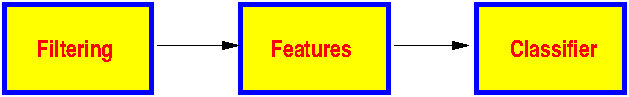
\includegraphics [width=0.5\linewidth] {bilder/bildchen.pdf}
\caption [Aufbau eines Mustererkennungssystems]{Aufbau eines Mustererkennungssystems und das Beispiel einer sehr langen Bildbeschreibung, die sehr ausführlich auf die Inhalte des Bildes zu sprechen kommt. \autocite{Oechsner2015}}
\label{fig:AufbauMustererkennungssystem}
\end{figure}

\begin{figure}
    \centering
    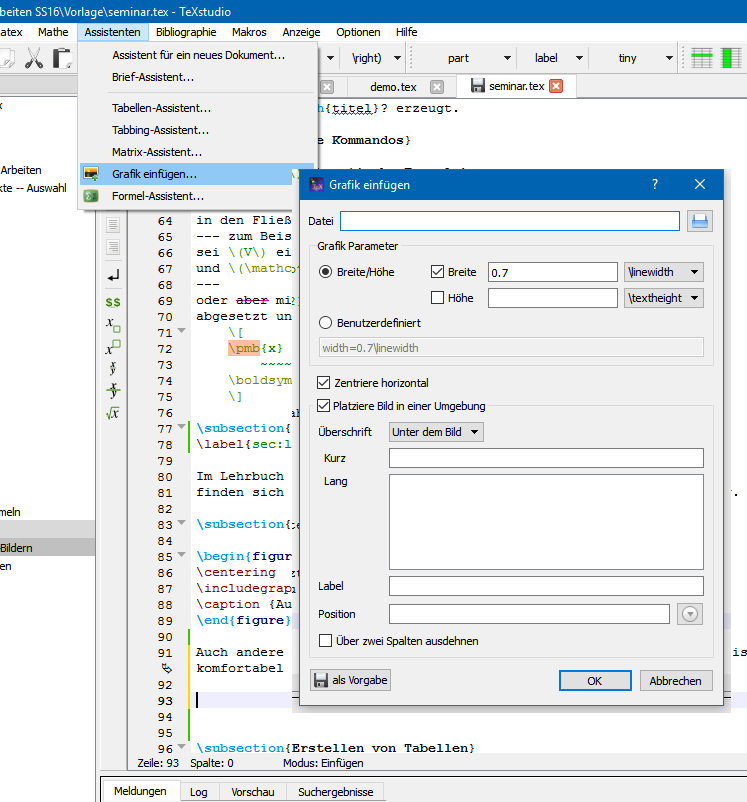
\includegraphics[width=0.5\linewidth] {bilder/GrafikEinfuegen.png}
    \caption{Hier die Bildunterschrift}
    \label{fig:my_label}
\end{figure}

Auch andere Grafikformate werden unterstützt. Verwenden Sie den Assistenten in TeXstudio, um komfortabel Grafiken einzufügen. Siehe dazu \autoref{fig:GrafikEinfuegen}. Die Grafiken finden sich nicht notwendigerweise direkt am Einfüge-Ort. Das Textsatzsystem richtet es so ein, dass es gut aussieht.

\begin{figure}
\centering
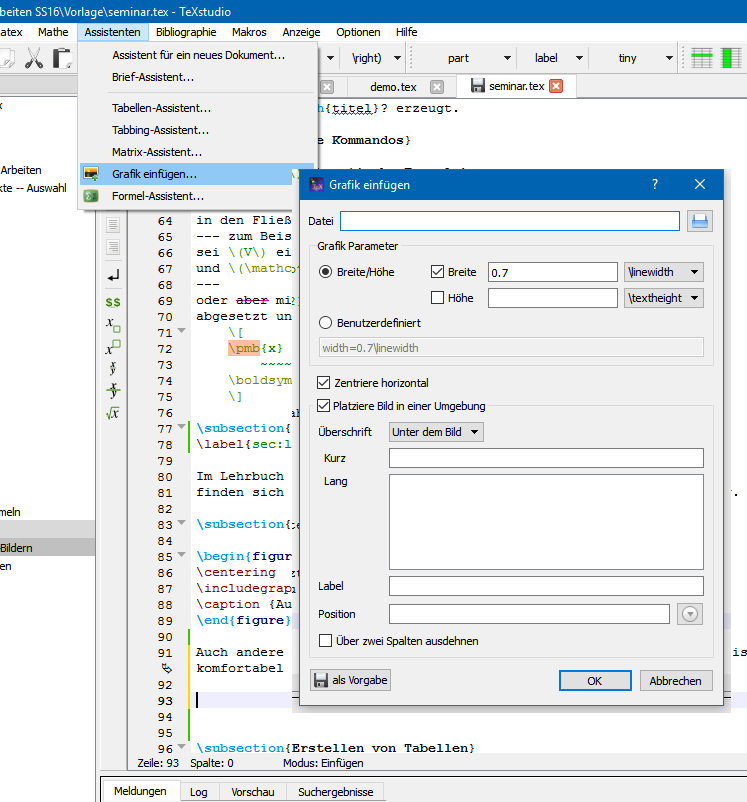
\includegraphics[width=0.7\linewidth]{bilder/GrafikEinfuegen}
\caption{Verwendung des Assistenten in \TeX studio, um eine Grafik einzufügen.}
\label{fig:GrafikEinfuegen}
\end{figure}

\subsection{Mehrere Bilder in einer Abbildung}

Manchmal ist es notwendig, mehrere Bilder in eine einzige Abbildung zu packen. Dazu kann man die \lstinline|subfigure|-Umgebung nutzen. Ein Beispiel dafür ist in \autoref{fig:subfigures} mit den Unterbildern \autoref{fig:subfig_1} und \autoref{fig:subfig_2} zu sehen. Der dazugehörige Code ist in der Vorlage und in \autoref{lst:subfigure} zu finden.

\begin{figure}
    \centering
    \begin{subfigure}{0.45\textwidth}
        \centering
        \missingfigure[figwidth=\textwidth]{Missing}
        \caption{Unterbild 1}
        \label{fig:subfig_1}
    \end{subfigure}
    \hfill
    \begin{subfigure}{0.45\textwidth}
        \centering
        \missingfigure[figwidth=\textwidth]{Missing}
        \caption{Unterbild 2}
        \label{fig:subfig_2}
    \end{subfigure}
    \caption{Gesamtbeschreibung der Unterbilder}
    \label{fig:subfigures}
\end{figure}

\begin{lstlisting}[language=TeX, float, caption={\LaTeX-Code für subfigures}, label={lst:subfigure}]
\begin{figure}
    \centering
    \begin{subfigure}{0.45\textwidth}
        \centering
        \missingfigure[figwidth=\textwidth]{Missing}
        \caption{Unterbild 1}
        \label{fig:subfig_1}
    \end{subfigure}
    \hfill
    \begin{subfigure}{0.45\textwidth}
        \centering
        \missingfigure[figwidth=\textwidth]{Missing}
        \caption{Unterbild 2}
        \label{fig:subfig_2}
    \end{subfigure}
    \caption{Gesamtbeschreibung der Unterbilder}
    \label{fig:subfigures}
\end{figure}
\end{lstlisting}

\section{Einbinden von Codeausschnitten}
Zur Verdeutlichung von Programmabläufen kann es hilfreich sein, Codeausschnitte darzustellen. In \LaTeX geht das über die \lstinline|lstlisting|-Umgebung des \lstinline|listings| Pakets:
\lstinputlisting[language={[LaTeX]TeX},nolol]{latex/lstlisting.tex}
\begin{lstlisting}[language=Python, float, caption={Simple Python program}, label={lst:python}]
if __name__ == "__main__":
    print("This is a listing")
\end{lstlisting}
Die Ausgabe des gezeigten Codeabschnitts ist in \autoref{lst:python} zu sehen.

\section{Abkürzungen}
\label{sec:Abkuerzungen}
Abkürzungen werden mit \lstinline|\ac{...}| in den Text geschrieben. Beispiel der ersten Verwendung: \ac{JSON}
Und ab der zweiten Verwendung: \ac{JSON}

Generell gilt: Abkürzungen nur dann verwenden, wenn dadurch die \emph{Lesbarkeit erhöht} wird.


\subsection{Querverweise}\label{sec:querverweise}
Verwenden Sie unter TeXstudio die rechte Maustaste in der Strukturübersicht, um für einen Abschnitt ein Label zu erzeugen, auf das Sie Bezug nehmen können (siehe \autoref{fig:LabelErzeugen}).

\begin{figure}
\centering
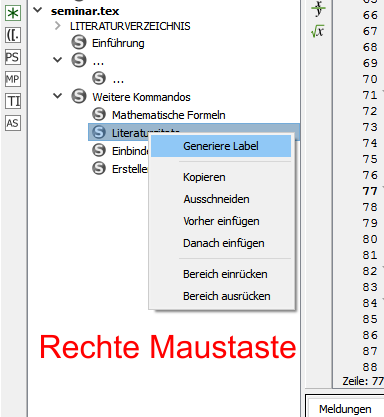
\includegraphics[width=0.4\linewidth]{bilder/LabelErzeugen}
\caption{Automatische Erzeugung eines Labels für Querverweise}
\label{fig:LabelErzeugen}
\end{figure}

Es wird ein Eintrag \verb|\label{key}| erzeugt, auf den man beispielsweise mit
\verb|\autoref{key}| verweisen kann. Verwendet man \verb|\autoref|, wird der Typ des Objekts
(z.\,B. Abbildung, Tabelle, etc.) mit ausgegeben. Verwendet man nur \verb|\ref|,
so wird nur die Nummerierung des Objekts ausgegeben. In den Anhang kann man darüber genauso verweisen: \autoref{sec:ThemaDesErstenAnhangs}, \autoref{fig:my_label_im_anhang}.

\subsection{Erstellen von Tabellen}

Das Volk hat gesprochen. Siehe \autoref{tab:tabular}. Auch hier kommt ein float zum Einsatz, jedoch mit dem Positionierungs-Hinweis \verb|[h]|. Jedes float sollte mit einem Label versehen werden, und es sollte im Text darauf verwiesen werden, da sich die Position ändern kann.

\begin{table}[h]
\centering
\begin{tabular} {|llc||r|}
	\hline
	Name & Rang & Fraktion & Stimmenanteil \\
	\hline
	Mobutu & General & CDU & 57\% \\
	Tsvangirai & Oberst & CSU & 63\% \\
	\hline
\end{tabular}
\caption {Bundestagswahl in Simbabwe}
\label{tab:tabular}
\end{table}

\autoref{tab:booktab} verwendet keine vertikalen Linien und entspricht dem üblicherweise in Büchern verwenden Stil. Derartige Tabellen sind deutlich ansehnlicher.

\begin{table}[h]
\centering
\begin{tabular} {llcr}
	\toprule
	Name & Rang & Fraktion & Stimmenanteil \\
	\midrule
	Mobutu & General & CDU & 57\% \\
	Tsvangirai & Oberst & CSU & 63\% \\
	\bottomrule
\end{tabular}
\caption {Bundestagswahl in Simbabwe}
\label{tab:booktab}
\end{table}

\subsection{Listen und Aufzählungen}

Listen und Aufzählungen werden in einer Umgebung angelegt (umschlossen von \verb|begin| und \verb|end|.). \verb|\begin{itemize}| leitet eine Liste ein und \verb|\begin{enumerate}| eine Aufzählung. Die Einträge werden jeweils mit \verb|\item| begonnen. Folgend zwei Beispiele.

Itemize:
\begin{itemize}
\item Test
\item Test
\item Test
\end{itemize}

Enumerate:
\begin{enumerate}
\item Test
\item Test
\item Test
\end{enumerate}

\subsection{Mathematische Formeln}

Mathematische Formeln werden mittels \verb|\(...\)|
in den Fließtext eingebaut
--- zum Beispiel \( E=mc^2 \) und:
sei \(V\) ein Vektorraum über \(\mathbb{R}\)
und \(\mathcal{M}\) eine Indexmenge
---
oder aber mittels \verb|\[...\]|
abgesetzt und zentriert dargestellt:
	\[
	\pmb{x} = \sqrt[3]{\frac{a^2-b^2}{a^2+b^2}}
		~~~~~ \text{versus} ~~~~~
	\boldsymbol{x} = \sqrt[3]{\frac{a^2-b^2}{a^2+b^2}}
	\]


\subsection{Silbentrennung}
Vertrauen Sie bitte nie einer automatischen Silbentrennung (auch nicht der von Microsoft Word \& Co.). In folgendem Test-Absatz ist das Wort "`Spracherkennung"' falsch getrennt.

Testzeile Testzeile Testzeile Testzeile Testzeile Testzeile Testzeile Testzeile Testzei Spracherkennung.

Sie können LaTeX die richtige Trennung mit \verb|\hyphenation{...}| mitteilen. Man tut das üblicherweise noch vor \verb|\begin{document}|.

\hyphenation{Sprach-er-ken-nung}	% hier jetzt zu Demonstrationszwecken im Text
Testzeile Testzeile Testzeile Testzeile Testzeile Testzeile Testzeile Testzeile Testzei Spracherkennung.



\section{Abschnitt im Kapitel zwei...}

\chapter{Kapitel 3}
\label{sec:Kapitel3}

Hier kommt eine Übersicht des dritten Kapitels hin.

\section{Abschnitt im Kapitel drei...}
\label{sec:abschnitt3.1}

\section{Abschnitt im Kapitel drei...}

\section{Abschnitt im Kapitel drei...}

\chapter{Zusammenfassung und Ausblick}
\label{sec:ZusammenfassungUndAusblick}

\blindtext

\section{Ausblick}
\label{sec:Ausblick}

Ein Ausblick...

\blindtext




%-----------------------------------------------------------------------------%
% Anhang                                                                      %
%-----------------------------------------------------------------------------%
\appendix

\chapter{Thema des ersten Anhangs}
\label{sec:ThemaDesErstenAnhangs}
Die Überschrift ist echt blöd gewählt...
\section{Der erste Abschnitt des ersten Anhangs}
Nach einer Überschrift kommt bekanntlich immer Text.

\begin{figure}
    \centering
    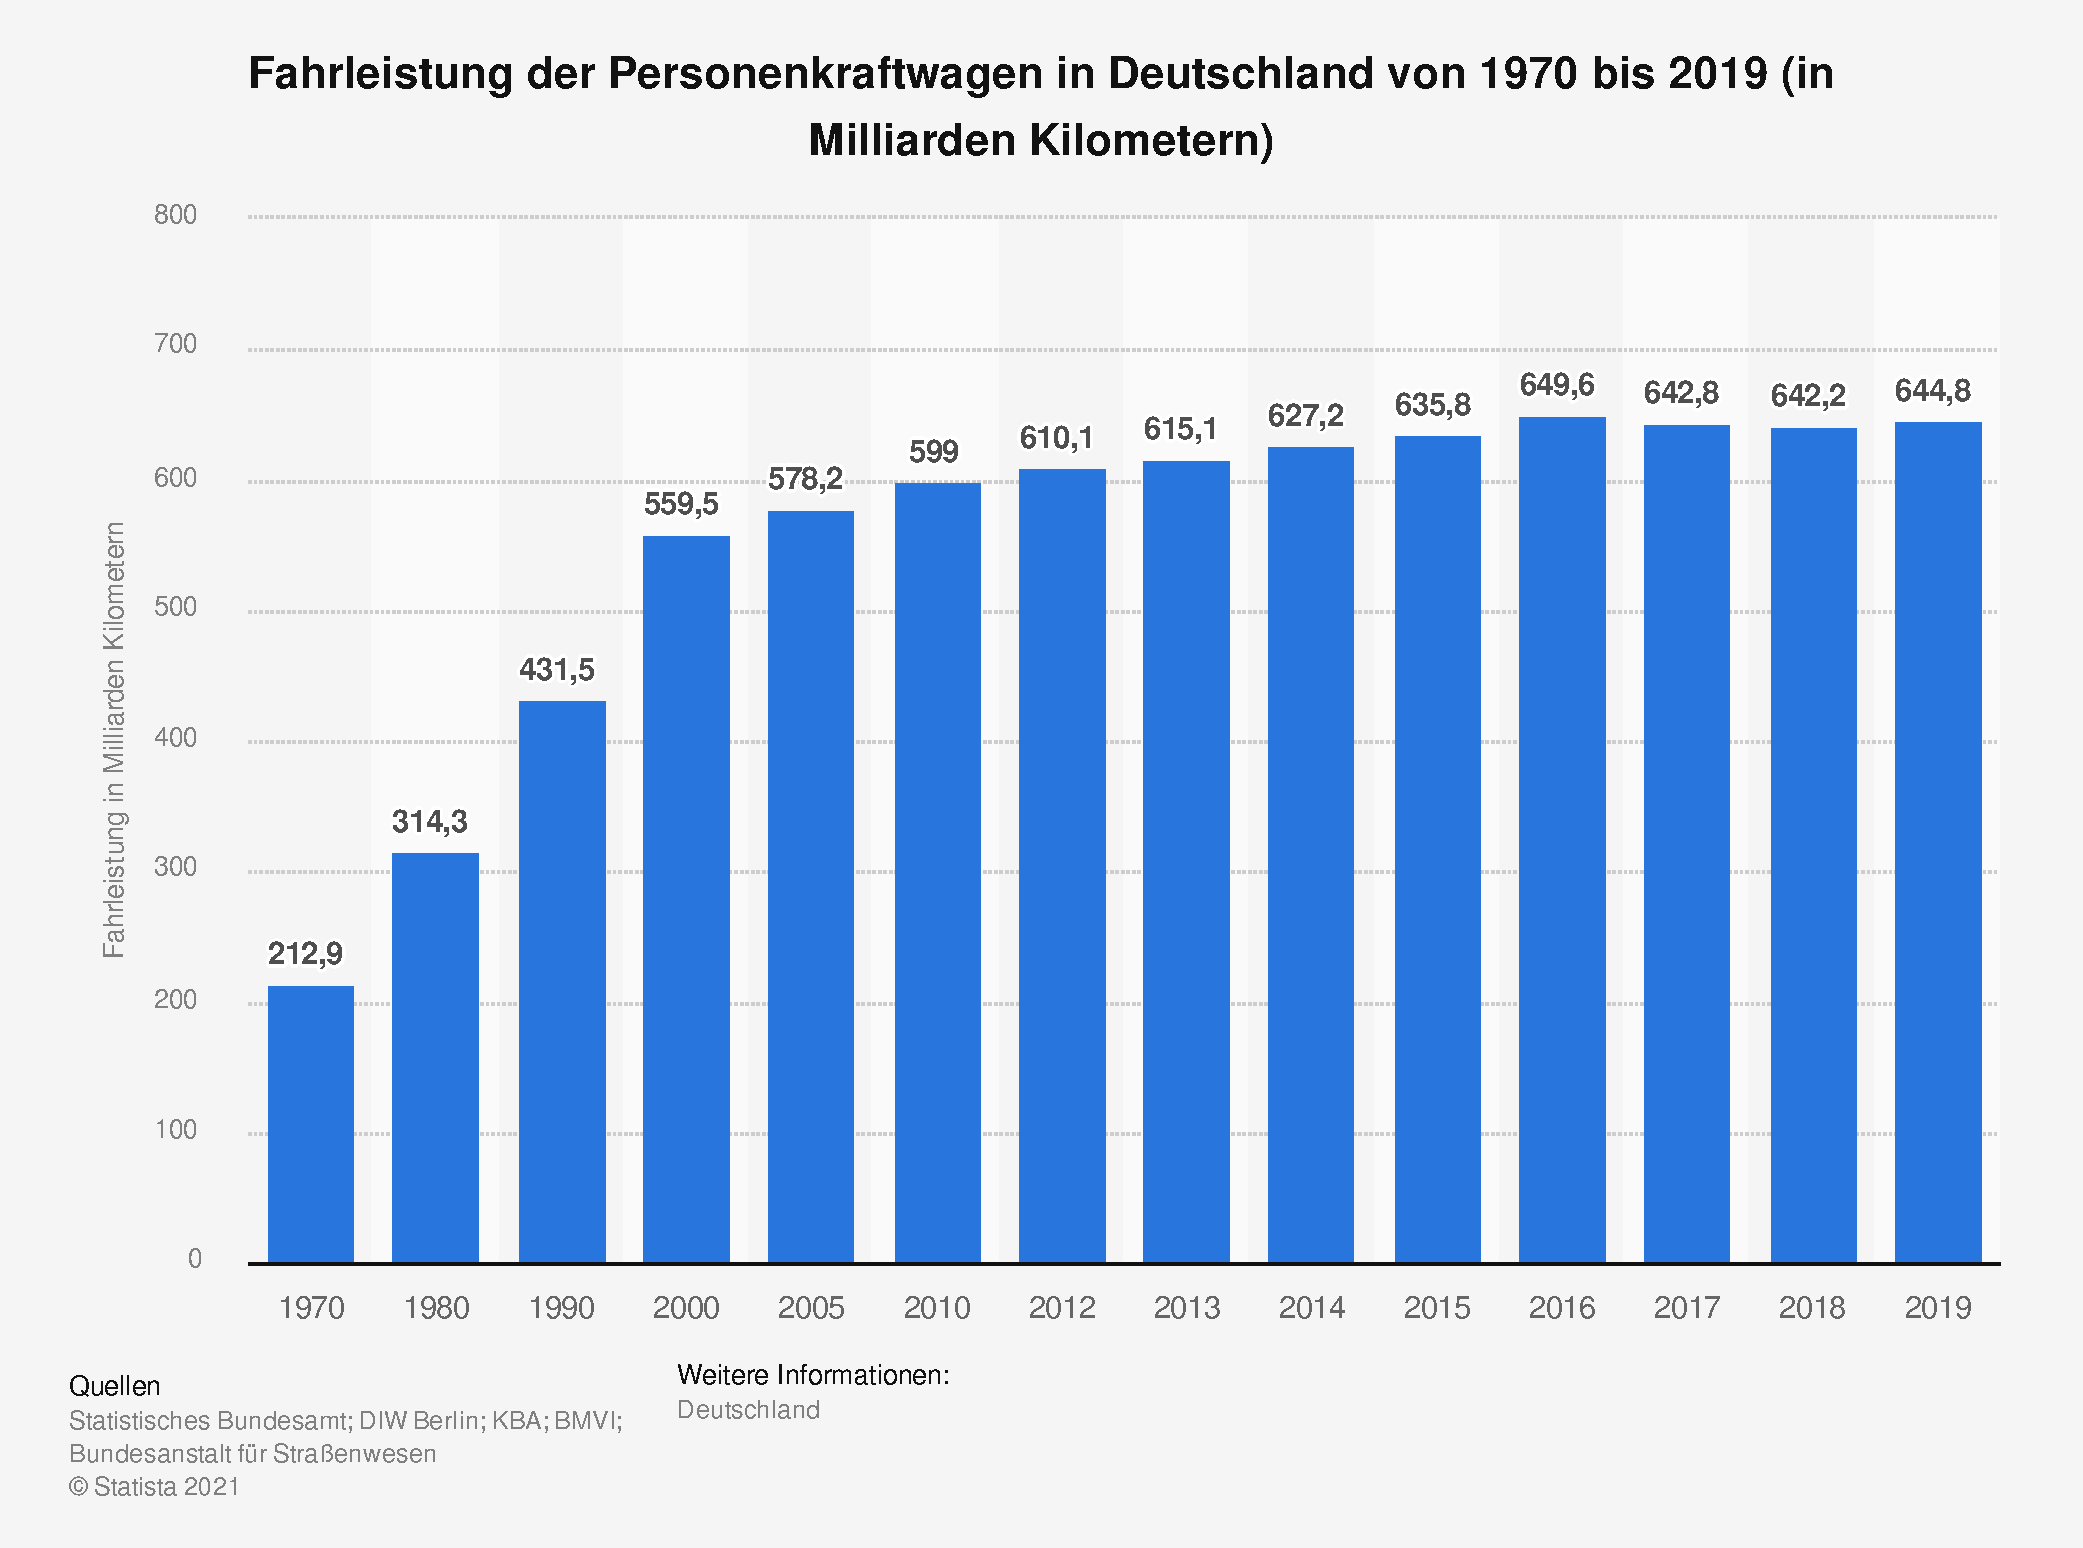
\includegraphics[width=1\linewidth]{bilder/statistic_id2984_fahrleistung-von-pkw-in-deutschland-bis-2019.pdf}
    \caption{Caption}
    \label{fig:my_label_im_anhang}
\end{figure}



\backmatter
%-----------------------------------------------------------------------------%
% Literaturverzeichnis                                                        %
%-----------------------------------------------------------------------------%
\cleardoublepage
% \printbibliography
% Hier kann das Literaturverzeichnis noch getrennt werden.
% Dafür ist zwingend biblatex notwendig!
\ohead[]{Literatur}
\printbibliography[nottype=misc]

\printbibliography[type=misc,title={Sonstige Quellen}]

\cleardoublepage
\ohead[]{\headmark}
\chapter*{Ehrenwörtliche Erklärung}

Hiermit versichere ich, dass die vorliegende Arbeit von mir selbstständig und ohne unerlaubte Hilfe angefertigt worden ist, insbesondere dass ich alle Stellen, die wörtlich oder annähernd wörtlich aus Veröffentlichungen entnommen sind, durch Zitate als solche gekennzeichnet habe. Ich versichere auch, dass die von mir eingereichte schriftliche Version mit der digitalen Version übereinstimmt. Weiterhin erkläre ich, dass die Arbeit in gleicher oder ähnlicher Form noch keiner Prüfungsbehörde / Prüfungsstelle vorgelegen hat. Ich erkläre mich damit \underline{einverstanden}/nicht einverstanden, dass die Arbeit der Öffentlichkeit zugänglich gemacht wird. Ich erkläre mich damit einverstanden, dass die Digitalversion dieser Arbeit zwecks Plagiatsprüfung auf die Server externer Anbieter hochgeladen werden darf. 
Die Plagiatsprüfung stellt keine Zurverfügungstellung für die Öffentlichkeit dar.



\vspace{2cm}

\noindent
(Ort, Datum)\hfill						(Eigenhändige Unterschrift)




\end{document}